\chapter{Implementation}\label{ch:5}

\newenvironment{ssfont}{\fontfamily{lmss}\selectfont}{\par}

The implementation is an evolution of previous web applications for the visualization of graph algorithms \cite{storz2013idp,velden2014idp,sefidgar2015idp,becker2015idp,zoennchen2015idp}. However, the requirements for graphs with arbitrary resources, a secondary visualization layer and high interactivity urged us to reimplement large parts of the existing codebase using different technologies while still maintaining the same look and feel. In the process, a complete understanding of the interplay between the different components was acquired, which allowed us to refactor them systematically. We improved code quality and maintainability by adhering to object oriented programming best practices of \textit{high cohesion and low coupling} \refFigure{fig:coh}. The separation of the components now fits the \textit{Model-View-Controller (MVC)} design pattern \refFigure{fig:mvc}, which was already applied partially in previous work, even better. 
\begin{figure}
\centering
\begin{subfigure}[b]{0.3\textwidth}
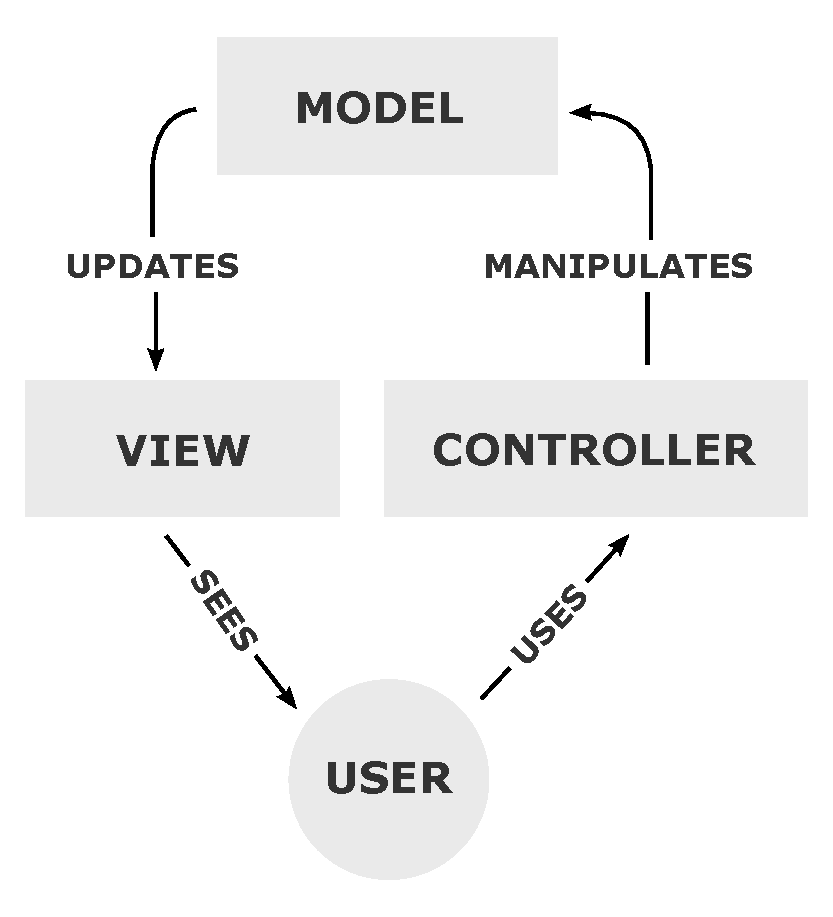
\includegraphics[width=\textwidth]{fig/MVC-Process}
	\caption{Model-View-Controller(MVC)\footnotemark}
	\label{fig:mvc}
\end{subfigure}
\begin{subfigure}[b]{0.68\textwidth}
\begin{small}
\begin{ssfont}
\begin{itemize}
\item Cohesion refers to the degree to which the elements of a class belong together, suggestion is all the related code should be close to each other, so we should strive for \textbf{high cohesion} and bind all related code together as far as possible. It has to do with the elements \textit{within} the class. %\textbf{High cohesion} means a class should do only one thing, but very well.
\item Coupling refers to the degree to which the different classes depend on each other, suggestion is all modules should be independent as far as possible, that's why \textbf{low coupling}. It has to do with the elements \textit{among} different classes. %\textbf{low coupling} suggest that class should have least possible dependencies.
\end{itemize}
\end{ssfont}
\end{small}
\caption{high cohesion, low coupling\footnotemark}
\label{fig:coh}
\end{subfigure}
\caption{Important design pattern and best practices in object oriented software engineering}
\label{fig:patterns}
\end{figure}
\footnotetext[1]{\url{https://en.wikipedia.org/wiki/Model-view-controller}}
\footnotetext{\url{http://stackoverflow.com/questions/14000762/what-does-low-in-coupling-and-high-in-cohesion-mean}}

%%http://www.xyzws.com/scjp/SGS11/5/2
%Loose coupling makes it possible to:
%\begin{itemize}
%	\item Understand one class without reading others
%	\item Change one class without affecting others
%	\item Thus: improves maintainability
%\end{itemize}
%
%High cohesion makes it easier to:
%\begin{itemize}
%	\item Understand what a class or method does
%	\item Use descriptive names
%	\item Reuse classes or methods
%\end{itemize}

These improvements make it easier to reuse and extend the code in other projects. Thus, an early prototype of our implementation already served as base for concurrent interdisciplinary projects \cite{fischer2016idp,feil2016idp}. These described some details of our implementation and its benefits over previous approaches. Here, we want to describe the overall concept and all improvements made in a unified manner to serve as a good starting point for future project. The chapter is organized into sections according to the MVC principle.

\section{Model}
%\item[Model] A major refactoring of the basic Graph class with the extension to arbitrary resources, easier algorithm state handling and new upload/download functionalities.
The graph Model of the previous work was not very clean and thus substantially refactored and simplified while new features were added. It contained code concerning the naming, colouring and layout of nodes and edges and methods to draw them on Canvas and to detect clicks using coordinate comparisons. However, the Model should be oblivious to the actual graph drawing and interactions, since these belong to the View or the Controller. Moreover, the previous graph Model only allowed for a single scalar weight to be defined on edges. We extended it so that an arbitrary number of resources can be defined on both the edges and the nodes. This was especially needed for the SPPTW. Furthermore we add an associative array to nodes and edges to store the changing algorithm state, easing the replay functionality.

The new Graph class, composed by its subclasses GraphNode and GraphEdge, achieves high cohesion as can be seen in the UML diagram \refFigure{fig:model}. The static serialization and deserialization methods \underline{parse} and \underline{stringify} were extended to support arbitrary resource vectors. In previous work, the serialization capabilities were unaccessible to the end user. We provide a link to download a graph in its textual representation, which is backwards compatible to the previous work. Additionally, a user can now locally upload a previously saved graph right from the browser using HTML5's FileReader capabilities. The previous raw ajax calls to load a saved sample graph from a server are now nicely wrapped in d3.text calls.

The loading of a graph, either from a local file or a remote server, is an asynchronous operation. According to \textit{MVC} \refFigure{fig:mvc}, the Model should update the View after any modifications to it, e.g. when another sample graph was selected or uploaded. We achieve \textit{low coupling} \refFigure{fig:coh} between the different components through the use of a static callback function registration method \underline{addChangeListener} \refFigure{fig:model}. All functions (of the View) that have been registered will be called after the graph has been loaded asynchronically without errors. To synchronize the current graph between GraphEditor and Algorithm, we employ a singleton pattern using the static Graph \underline{instance}.


\renewcommand{\umldrawcolor}{black}

\colorlet{lightyellow}{yellow!20} %default color
\renewcommand{\umlfillcolor}{lightyellow}

\begin{figure}
\centering
\begin{tikzpicture}
  \begin{class}[text width=7cm]{Graph}{0,0}
    \attribute{\underline{instance} : Graph}
    %\attribute{\underline{onLoadedCbFp} : [function]}
    \operation{getNodes() : [GraphNode]}
    \operation{getEdges() : [GraphEdge]}
    \operation{\underline{stringify(graph : Graph)} : String}
    \operation{\underline{parse(text : String)} : Graph}
    \operation{\underline{addChangeListener(callbackFp : function)}}
    %\operation{\underline{loadInstance(fileurl : String)}}
    %\operation{\underline{handleFileSelect(filename : String)}}
  \end{class}
  
  \begin{class}[text width=5.5cm]{GraphNode}{-5,-5}
    \attribute{resources : []}
    \attribute{state : \{\}}
    \attribute{x : number}
    \attribute{y : number}
    \operation{getInEdges() : [GraphEdge]}
    \operation{getOutEdges() : [GraphEdge]}
  \end{class}
  
  \begin{class}[text width=5.5cm]{GraphEdge}{4,-5}
    \attribute{resources : []}
    \attribute{state : \{\}}

    \operation{getStartNode() : GraphNode}
    \operation{getEndNode() : GraphNode}
  \end{class}
  
  \begin{class}[text width=3cm]{ResidualEdge}{1,-10}
  \end{class}
  
  \begin{class}[text width=2cm]{Label}{6,-10}
  \end{class}
  
  \composition{Graph}{nodes}{*}{GraphNode}
  \composition{Graph}{edges}{*}{GraphEdge}
  \association{GraphNode}{start,end}{1}{GraphEdge}{*}{in,out}
  
  \unidirectionalAssociation{GraphNode}{eligible}{*}{ResidualEdge}
  \association{GraphEdge}{}{1}{ResidualEdge}{1..2}{}
  \association{Label}{resident}{*}{GraphNode}{resident}{1}
  \unidirectionalAssociation{Label}{path}{*}{GraphEdge}

\end{tikzpicture}
\caption{UML class diagram for the Model. From a high-level perspective, we model a Graph as a composition of nodes and edges with associations between these two entities reflecting the network structure: Each GraphEdge has a start and an end node, while each GraphNode has an arbitrary number of incoming and outgoing edges. Arrays for resources denoted by [] and associate arrays for state variables denoted by \{\} are attributes of both nodes and edges. Static attributes and method are \underline{underlined}. ResidualEdge and Label are two concepts that we needed for the implementation of our Algorithms. These are primarily associated with GraphEdge, either 1:1 or 2:1 for the first or 1:n for the latter. For performance reason, we also established associations with GraphNode. A GraphNode can be queried for all its current outgoing eligible ResidualEdges, which is needed for applying a push operation. Label and GraphNode are associated bidirectionally: a Label needs to know its resident vertex so it can check path extensions easily for feasibility using the time-window of the vertex, while a GraphNode can be queried for all the Labels ending in it so we can apply dominance rules to them.}
\label{fig:model}
\end{figure}



\section{View}
%\item[View] A complete rewrite of the abstract GraphDrawer class for network visualization using D3.js and SVG instead of Canvas with the possibility to download it in vector format at any time. A Logger utility which allows to log algorithm execution messages with up to 3 indentation levels.
 A complete rewrite of the graph visualization code using D3.js and SVG instead of Canvas. This is the GraphDrawer class, which should be used as a base class. Customization is easily possible by overwriting methods that will be called from inside of D3.js data join. Any visualization can be saved to disk in png or svg format, for which styles and marker definitions are automatically inlined. A Logger utility which allows to log algorithm execution messages with up to 3 indentation levels. This is very useful for development, but also for the final algorithm so people can trace the algorithm execution.


\colorlet{lightgreen}{Akzent-Gruen!50}%tumblue3!40!lightyellow} %default color
%accentuating green} %SpringGreen}

\begin{figure}
\centering
\hspace*{-1.5cm}%
\begin{tikzpicture}
  \renewcommand{\umlfillcolor}{tumblue4} %accentuating light blue}

  \begin{abstractclass}[text width=8cm]{GraphDrawer}{-3,0}
    \attribute{svg : <svg>}
    \operation{onNodesEntered(selection : [])}
    \operation{onNodesUpdated(selection : [])}
    \operation{onEdgesEntered(selection : [])}
    \operation{onEdgesUpdated(selection : [])}
    \operation{edgeText(d : GraphEdge) : String}
    \operation{nodeText(d : GraphNode) : String}
    \operation{nodeLabel(d : GraphNode) : String}
  \end{abstractclass}

  
  \begin{class}[text width=2.8cm]{LabelDrawer}{-4.9,-6}
  \end{class}
 
  \begin{class}[text width=5cm]{ResidualGraphDrawer}{3.5,-6}
  	\inherit{GraphDrawer}
  \end{class}
  

  \begin{class}[text width=2cm]{Logger}{-1,-6}
  \end{class}
  
  \renewcommand{\umlfillcolor}{lightgreen}
  
  \begin{class}[text width=3cm]{GraphEditor}{-8.5,-8}
    	\inherit{GraphDrawer}
  \end{class}
  
  \begin{class}[text width=5cm]{LabelSettingAlgorithm}{-3,-8}
  	\inherit{GraphDrawer}
  \end{class}

  \begin{class}[text width=5cm]{PushRelabelAlgorithm}{3,-8}
  	\inherit{GraphDrawer}
  \end{class}
  
  \begin{abstractclass}[text width=2.5cm]{Tab}{-3,-11}
  	\operation{init()}
  	\operation{activate()}
  	\operation{deactivate()}
  \end{abstractclass}
  
  \begin{class}[text width=3.5cm]{GraphEditorTab}{-7.5,-10}
    \inherit{Tab}
  	\operation{setGraphHandler()}
  \end{class}
  
  \begin{class}[text width=3.5cm]{AlgorithmTab}{2,-10}
    \inherit{Tab}
  	\operation{startFastForward()}
  	\operation{stopFastForward()}
  \end{class}
  
  \aggregation{LabelSettingAlgorithm}{}{}{LabelDrawer}
  \aggregation{PushRelabelAlgorithm}{}{}{ResidualGraphDrawer}
  
  
  \unidirectionalAssociation{AlgorithmTab}{}{}{Logger}
  \unidirectionalAssociation{LabelSettingAlgorithm}{}{}{AlgorithmTab}
  \unidirectionalAssociation{PushRelabelAlgorithm}{}{}{AlgorithmTab}
  \unidirectionalAssociation{GraphEditor}{}{}{GraphEditorTab}


\end{tikzpicture}
\caption{UML class diagram for View (blue) and Controller (green). The multiplicities are all 1:1 and thus not drawn. The abstract base class GraphDrawer of the View forms the basis for all graph-based visualizations. The Logger and the secondary visualization layers LabelDrawer and ResidualGraphDrawer are part of the View, but only the latter one displays a graph (with the possibility to change the axes) and thus extends the GraphDrawer. The abstract base class Tab of the Controller is extended to form a GraphEditorTab and an AlgorithmTab. Finally, the actual GraphEditor and the two implemented Algorithms are associated with a Tab while inheriting from the GraphDrawer. Each Algorithm has a secondary visualization layer, we model this relationship with an aggregation.}
\end{figure}


\section{Controller}
%\item[Controller] A new GraphEditor with support for modifying graphs with an arbitrary number of resources on nodes and edges easily. A small refactoring improved future code reusability and simplified the reverse functionality and the synchronization between algorithm state and pseudocode lines.
	A new way to save stateful data of the graph using JSON.stringify, which makes implementing the reverse functionality much easier. A new way to synchronize between the algorithm state (in the sense of a finite state machine), pseudocode lines, and their description using d3.
